\subsubsection*{Inicialización de la MMU}

\par Al inicializar la MMU, tenemos dos tareas que hacer: inicializar la direcci\'on donde se encuentra la pr\'oxima p\'agina libre y mapear el directorio del kernel(descripto en el Ejercicio 3). Luego, a medida que se pide la siguiente p\'agina, aumentamos esta variable en 4kb (una p\'agina) para obtener la direcci\'on de la siguiente.

\begin{lstlisting} [caption={Contador de Páginas Libres}],label=mmucontador] 
unsigned int proxima_pagina_libre;

void mmu_inicializar() {
  inicializar_kernel_mapping();
  proxima_pagina_libre = INICIO_PAGINAS_LIBRES;
}

unsigned int mmu_proxima_pagina_fisica_libre() {
    unsigned int pagina_libre = proxima_pagina_libre;
	proxima_pagina_libre += PAGE_SIZE;
	return pagina_libre;
}
\end{lstlisting}

\subsubsection*{Mapeo y Desmapeo de P\'aginas}

\par Los algoritmos de mapeo y desmapeo se pueden entender con mayor facilidad con el siguiente diagrama:

\begin{figure}[ht!]
\centering
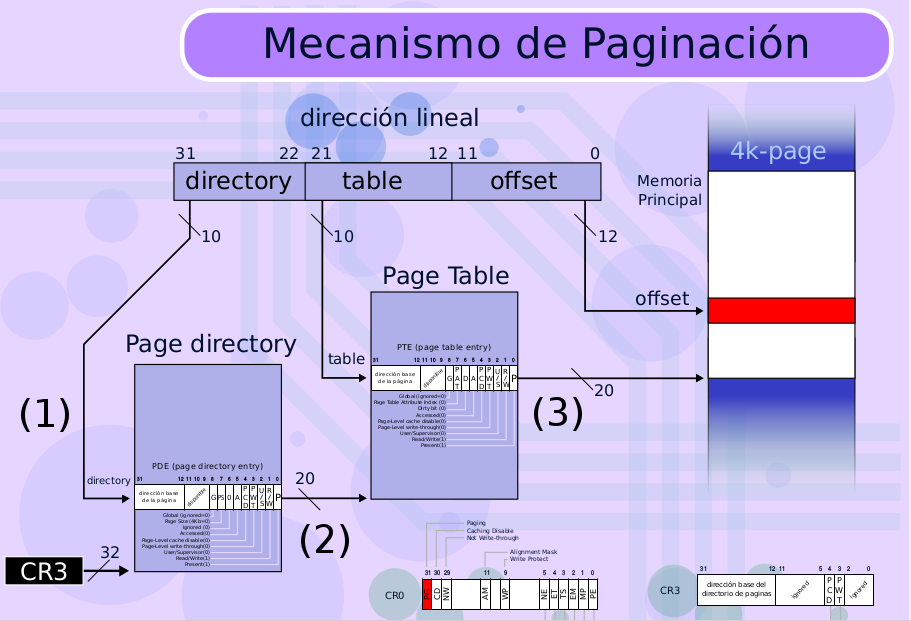
\includegraphics[width=100mm]{imagenes/paginacion.png}
\caption{Mapeo de P\'aginas}
\end{figure}

\par Para mapear p\'aginas \texttt{mmu_map_page} toma una direcci\'on virtual, una f\'isica, un selector del directorio a mapear, y dos par\'ametros de permisos (user/supervisor, read/write).

\par El algoritmo de mapeo es el siguiente:

\begin{itemize}
\item Primero limpiamos los bits de permisos del selector y obtenemos el directorio.
\item  Luego buscamos la tabla de p\'aginas para mapear. Para esto avanzamos hasta su descriptor sumando a la direcci\'on base el offset indicado en los primeros 10 bits de la direcci\'on virtual.
\item Si dicho descriptor tiene el bit presente en 1, shifteamos su base y obtenemos la direcci\'on del comienzo de la tabla que buscamos; sino, creamos la tabla y asignamos su base al descriptor del directorio.
\item Finalmente avanzamos hasta el descriptor de la p\'agina, seteamos el bit de presente junto con los dem\'as permisos y su base ser\'a la direcci\'on f\'isica shifteada 12 a la derecha.
\end{itemize}

\begin{lstlisting} [caption={Mapeo de p\'aginas}],label=mmuMapPage] 
void mmu_map_page(unsigned int virtual, unsigned int cr3, unsigned int fisica, char sup, char rw){
	page_directory_entry* page_dir = (page_directory_entry*) ((cr3 >> 3) << 3);

	page_table_entry* pte;
	if (page_dir[PDE_INDEX(virtual)].p){
		pte = (page_table_entry*) (page_dir[PDE_INDEX(virtual)].base << 12);
	} else {
		pte = (page_table_entry*) mmu_proxima_pagina_fisica_libre();
		page_dir[PDE_INDEX(virtual)].base = ((unsigned int) pte) >> 12;
		page_dir[PDE_INDEX(virtual)].p = 1;
		page_dir[PDE_INDEX(virtual)].rw = 1;
		page_dir[PDE_INDEX(virtual)].s = 1;
	}
	pte[PTE_INDEX(virtual)].p = 1;
	pte[PTE_INDEX(virtual)].rw = rw;
	pte[PTE_INDEX(virtual)].s = sup;
	pte[PTE_INDEX(virtual)].pwt = 0;
	pte[PTE_INDEX(virtual)].pcd = 0;
	pte[PTE_INDEX(virtual)].a = 0;
	pte[PTE_INDEX(virtual)].d = 0;
	pte[PTE_INDEX(virtual)].pat = 0;
	pte[PTE_INDEX(virtual)].g = 0;
	pte[PTE_INDEX(virtual)].disp = 0;
	pte[PTE_INDEX(virtual)].base = fisica >> 12;		
	tlbflush();
}
\end{lstlisting}

\par \texttt{mmu_unmap_page} toma la direcci\'on virtual y el cr3 del directorio. Para desmapear accedemos al descriptor de dicha p\'agina y seteamos el bit de presente en 0.

\begin{lstlisting} [caption={Desmapeo de p\'aginas}],label=mmuUnmap] 
void mmu_unmap_page(unsigned int virtual, unsigned int cr3){
	page_directory_entry* page_dir = (page_directory_entry*) ((cr3 >> 3) << 3);
	page_table_entry* pte = (page_table_entry*) (page_dir[PDE_INDEX(virtual)].base << 12);
	pte[PTE_INDEX(virtual)].p = 0;
}
\end{lstlisting}

\newpage
\subsubsection*{Inicialización de directorios y tablas para Zombis}

\par \texttt{mmu_inicializar_dir_zombi} toma el tipo de zombie que el jugador quiere inicializar y la posici\'on (x,y) donde se quiere inicializarlo y devuelve la direcci\'on del directorio creado para este zombi.

\par La inicializaci\'on del directorio y tabla de p\'aginas para dicho zombi respetan el formato presentado en el enunciado:

\begin{figure}[ht!]
\centering
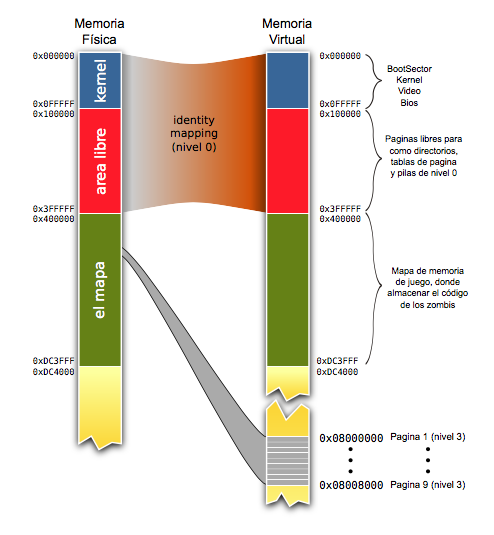
\includegraphics[width=100mm]{imagenes/memoriatarea.png}
\caption{Mapa de memoria de la Tarea.}
\end{figure}

\par La descripci\'on del algoritmo es la siguiente:

\begin{itemize}
\item Para obtener el nuevo directorio, pedimos una p\'agina libre y mapeamos con identity mapping todas las p\'aginas entre 0x000000 y 0x03FFFFF.
\item Luego, obtenemos la direcci\'on f\'isica a la que corresponde esa posici\'on (entre 0x400000 y 0xDC3FFF) y copiamos el c\'odigo del zombi (que dependiendo del tipo, est\'a en alguna direcci\'on f\'isica fija). Cabe aclarar que primero mapeamos en el directorio del kernel la p\'agina destino (que no est\'a mapeada), y luego de copiar el c\'odigo la desmapeamos.
\item Por \'ultimo, mapeamos las 9 p\'aginas virtuales del zombi a sus correspondientes f\'isicas.
\end{itemize}

\newpage
\begin{lstlisting} [caption={Inicializaci\'on directorio y tabla de p\'aginas del zombi}],label=mmuDirZombi] 
unsigned int mmu_inicializar_dir_zombi(unsigned short x, unsigned short y, zombie z) {
	page_directory_entry* dir_pagina = (page_directory_entry*) mmu_proxima_pagina_fisica_libre();
	inicializar_con_identity_mapping(dir_pagina);

	unsigned int* origin;
	switch (z) {
		case A_MONK:
			origin = (unsigned int*)0x10000;
			break;
        case A_SUICIDE_UNIT:
        	origin = (unsigned int*)0x11000;
        	break;
        case A_DRUNK_DRIVER:
        	origin = (unsigned int*)0x12000;
        	break;
        case B_MONK:
        	origin = (unsigned int*)0x13000;
        	break;
        case B_SUICIDE_UNIT:
        	origin = (unsigned int*)0x14000;
        	break;
        case B_DRUNK_DRIVER:
        	origin = (unsigned int*)0x15000;
        	break;
    }

	unsigned int* dest = (unsigned int*) mmu_get_map_position(x, y); 
	mmu_map_page((unsigned int)dest, rcr3(), (unsigned int)dest, 0, 1);
	unsigned int i;
	for (i=0; i<1024; i++){
		dest[i] = origin[i];
	}
	
	mmu_unmap_page((unsigned int)dest, rcr3());

	if (x == POS_INIT_ZOMBI_A){
		mmu_map_adjacent_to_zombi(0, (unsigned int) dir_pagina, x, y);
	} else if (x == POS_INIT_ZOMBI_B){
		mmu_map_adjacent_to_zombi(1, (unsigned int) dir_pagina, x, y);
	}

	return (unsigned int)dir_pagina;
}
\end{lstlisting}

\par Para manejar el video convenientemente, nos pareci\'o \'util hacer una funci\'on para obtener la p\'agina del video asociada a una coordenada.

\begin{lstlisting} [caption={Obtener p\'agina de coordenada}],label=mmuObtenerPaginaDedir] 
unsigned int mmu_get_map_position ( int x,  int y) {
	return 0x400000 + (MOD(y,44) * 78 + x) * PAGE_SIZE;
}
\end{lstlisting}

\newpage
\par Finalmente, \texttt{mmu_map_adjacent_to_zombi} mapea las 9 p\'aginas virtuales del zombie a las 9 p\'aginas f\'isicas del video.

\begin{lstlisting} [caption={Mapeo de zombi a una coordenada en el mapa}],label=mmuMapDirZombi] 
void mmu_map_adjacent_to_zombi(unsigned int player, unsigned int dir_pagina, unsigned int x, unsigned int y){
	mmu_map_page(VIRTUAL_COD_ZOMBIE_1, dir_pagina, mmu_get_map_position(x, y), 1, 1);
	if (player == 0) {
		mmu_map_page(VIRTUAL_COD_ZOMBIE_2, dir_pagina, mmu_get_map_position(x+1, y), 1, 1);
		mmu_map_page(VIRTUAL_COD_ZOMBIE_3, dir_pagina, mmu_get_map_position(x+1, y+1), 1, 1);
		mmu_map_page(VIRTUAL_COD_ZOMBIE_4, dir_pagina, mmu_get_map_position(x+1, y-1), 1, 1);
		mmu_map_page(VIRTUAL_COD_ZOMBIE_5, dir_pagina, mmu_get_map_position(x, y+1), 1, 1);
		mmu_map_page(VIRTUAL_COD_ZOMBIE_6, dir_pagina, mmu_get_map_position(x, y-1), 1, 1);
		mmu_map_page(VIRTUAL_COD_ZOMBIE_7, dir_pagina, mmu_get_map_position(x-1, y), 1, 1);
		mmu_map_page(VIRTUAL_COD_ZOMBIE_8, dir_pagina, mmu_get_map_position(x-1, y-1), 1, 1);
		mmu_map_page(VIRTUAL_COD_ZOMBIE_9, dir_pagina, mmu_get_map_position(x-1, y+1), 1, 1);
	} else {
		mmu_map_page(VIRTUAL_COD_ZOMBIE_2, dir_pagina, mmu_get_map_position(x-1, y), 1, 1);
		mmu_map_page(VIRTUAL_COD_ZOMBIE_3, dir_pagina, mmu_get_map_position(x-1, y-1), 1, 1);
		mmu_map_page(VIRTUAL_COD_ZOMBIE_4, dir_pagina, mmu_get_map_position(x-1, y+1), 1, 1);
		mmu_map_page(VIRTUAL_COD_ZOMBIE_5, dir_pagina, mmu_get_map_position(x, y-1), 1, 1);
		mmu_map_page(VIRTUAL_COD_ZOMBIE_6, dir_pagina, mmu_get_map_position(x, y+1), 1, 1);
		mmu_map_page(VIRTUAL_COD_ZOMBIE_7, dir_pagina, mmu_get_map_position(x+1, y), 1, 1);
		mmu_map_page(VIRTUAL_COD_ZOMBIE_8, dir_pagina, mmu_get_map_position(x+1, y+1), 1, 1);
		mmu_map_page(VIRTUAL_COD_ZOMBIE_9, dir_pagina, mmu_get_map_position(x+1, y-1), 1, 1);
	}
}
\end{lstlisting}